% !TeX spellcheck = en_GB

\chapter{A note on laser safety}

The \SI{775}{nm} line is a class 4 laser source. Under normal operation, the user is protected from it. However, when calibrating the STED beam or placing new components in the beam path, it is theoretically possible for the collimated laser beam to be reflected into the user's eyes. A high-powered laser beam can do permanent damage to the skin and retina, so we have to make sure we stay below the limits imposed by the Work Environment Agency's (Arbetsmiljöverkets) limits \cite{AFS2009:7}. These regulations set forth three main conditions to calculate the Maximum Permissible Exposure (MPE) of a pulsed laser, see table 2.6 of the regulations. Important values and formulas about our setup, as well as the limits provided by the Work Environment Agency are provided in \autoref{tab:laser-safety} and in the text below.

\begin{table}[h]
	\centering
	\caption{Operating characteristics of the 775 laser line and relevant safety parameters. }
	\begin{tabular}{lll}
		\toprule
		Quantity                   & Symbol               & Value                 \\ \midrule
		Beam radius                & $ r $                & 0.5 mm                \\
		Pulse width (FWHM)         & $ \tau $             & 1.3 ns                \\
		Pulse repetition frequency & $ f $                & 40 MHz                \\
		Pulse energy               & $ E_\mathit{pulse} $ & 31 nJ                 \\
		Average power              & $P_\mathit{avg} $    & 1.25 W                \\ \\
		Thermal correction time    & $ T_\mathit{min} $   & 18 \si{\micro\second} \\
		Ca                         & $ C_a $              & 1.41                  \\
		Cc                         & $ C_c $              & 1                     \\
		Ce                         & $ C_e $              & 1                     \\ \bottomrule
	\end{tabular}
	\label{tab:laser-safety}
\end{table}

\paragraph{Rule 1: The dose of a single pulse must not exceed the single-pulse MPE.} The pulse dose $ H_\mathit{pulse} $ of the 775~nm laser at full power is
\begin{equation}
	H_\mathit{pulse} = \frac{E_\mathit{pulse}}{2\pi r^2} \approx \SI{39}{mJ/m^2},
\end{equation}
whereas the MPE equals
\begin{equation}
	H_\mathit{pulse}^\mathit{MPE} = \num{5e-3} C_a C_e = \SI{7.1}{mJ/m^2}.
\end{equation}
This formula is found in table 2.2 of the regulations.

\paragraph{Rule 2: The dose of a single pulse may not exceed the thermally-corrected MPE.} This weighs the pulse MPE with the amount of pulses in an interval $ T_\mathit{min} $. The number of pulses in such an interval is $ n = f\cdot T_\mathit{min} $, so
\begin{equation}
	H_\mathit{thermal}^\mathit{MPE} =  n^{-1/4} H_\mathit{pulse}^\mathit{MPE} = \SI{1.3}{mJ/m^2}.
\end{equation}
Rule 2 is therefore more strict than the rule 1. For safe operation, the laser must be ran at a power below 3.3\% $ (=H^\mathit{MPE}_\mathit{thermal} / H_\mathit{pulse}) $.

\paragraph{Rule 3: The cumulative dose for a group of pulses in an interval of time t must not exceed the MPE for a single pulse of that time.} Taking the necessary values from tables 2.2 and 2.3, the cumulative MPE is defined as
\begin{equation}
	H_\mathit{tot}^\mathit{MPE}(t) = \left\{\begin{array}{rl}
		\num{5e-3} \:C_a C_e &  t<\SI{18}{\mu s,} \\
		18 t^{0.75} \:C_a C_e &  \SI{18}{\mu s} < t < \SI{10}{s}, \\
		10 t\:C_a C_c  &t> \SI{10}{s}.
	\end{array}\right.
\end{equation}
The actual dose, on the other hand, is
\begin{equation}
	H_\mathit{tot}(t) = \lfloor ft \rfloor H_\mathit{pulse},
\end{equation}
where $ \lfloor \cdot \rfloor$ is the flooring function. This function is plotted in \autoref{fig:laser-safety-mpe}, from which it can be seen that the laser is only safe to use at 0.0005\% capacity. Since the minimum laser power offered by the software is .05\%, OD2 goggles should be worn to guarantee safe operation of the 775~nm laser.

\begin{figure}
	\centering
	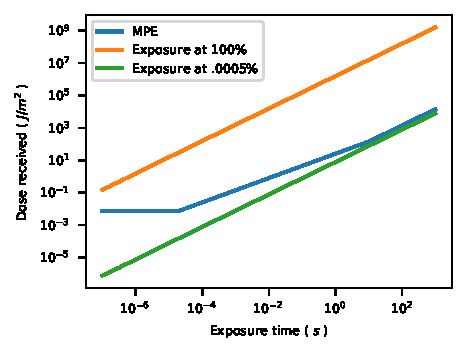
\includegraphics{laser_safety.pdf}
	\caption{Maximum permissible  and actual exposure to the collimated STED beam as a function of exposure time.}
	\label{fig:laser-safety-mpe}
\end{figure}